%nope, thjat's wrong. need to cleanup halt class *once*

\subsection{Cleaner Resurrection}

The student had the very good reflex to use \textit{haltOnce} rather than \textit{halt}.
This means that the breakpoint should trigger only once (Figure~\ref{fig:prefix}).
This is achieved by putting an association inside the additional state of the compiled method.
A cleaner solution would have been to just replace the boolean to deactivate the halt~\ref{fig:postfix}.
Again, doing this with Polyphemus is very easy.

However, it only occurred to us after the image was already resurrected !


\begin{figure}[h]
    \centering
    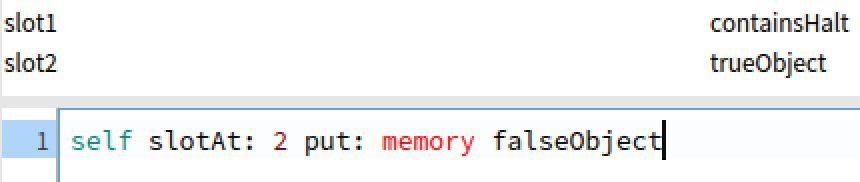
\includegraphics[width=0.7\linewidth]{prefix}
    \caption{
    Method state keeping the haltOnce state.
    This breakpoint is activated
    }%
    \label{fig:prefix}
\end{figure}


\begin{figure}[h]
    \centering
    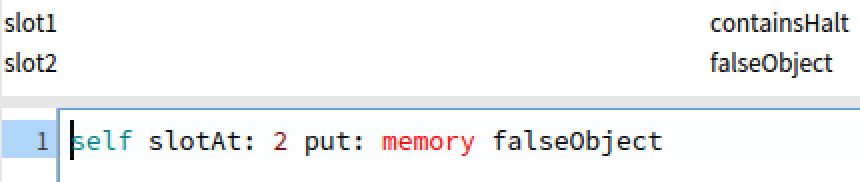
\includegraphics[width=0.7\linewidth]{postfix}
    \caption{
    Fix method state keeping the haltOnce state.
    This breakpoint is now deactivated.
    }%
    \label{fig:postfix}
\end{figure}
